\section{BCI NextMind}

El BCI NextMind\footnote{NextMind: \url{https://ar.snap.com/welcome-nextmind}} como se ha mencionado anteriormente es una interfaz cerebro-computador revolucionaria. El dispositivo se presenta en forma de un casco compacto y ligero, diseñado y pensado para la comodidad y facilidad de uso del usuario.



El dispositivo NextMind se caracteriza por su diseño inalámbrico, lo que facilita la movilidad y mejora la comodidad del usuario. Este casco viene con una banda ajustable mediante una cinta de velcro, lo que permite adaptarse a diferentes tamaños y formas de cabeza, garantizando así su accesibilidad y funcionalidad para una amplia diversidad de usuarios.



NextMind se distingue por sus nueve electrodos colocados estratégicamente para capturar las señales electroencefalográficas (EEG) desde el lóbulo occipital del cerebro. Estos electrodos registran las respuestas neuronales provenientes de los ``neurotags'' visuales y envía la respuesta a la computadora del usuario (véase en la figura \ref{figure:nextmind-electrodes})

\begin{figure}[!htb]
   \centering
    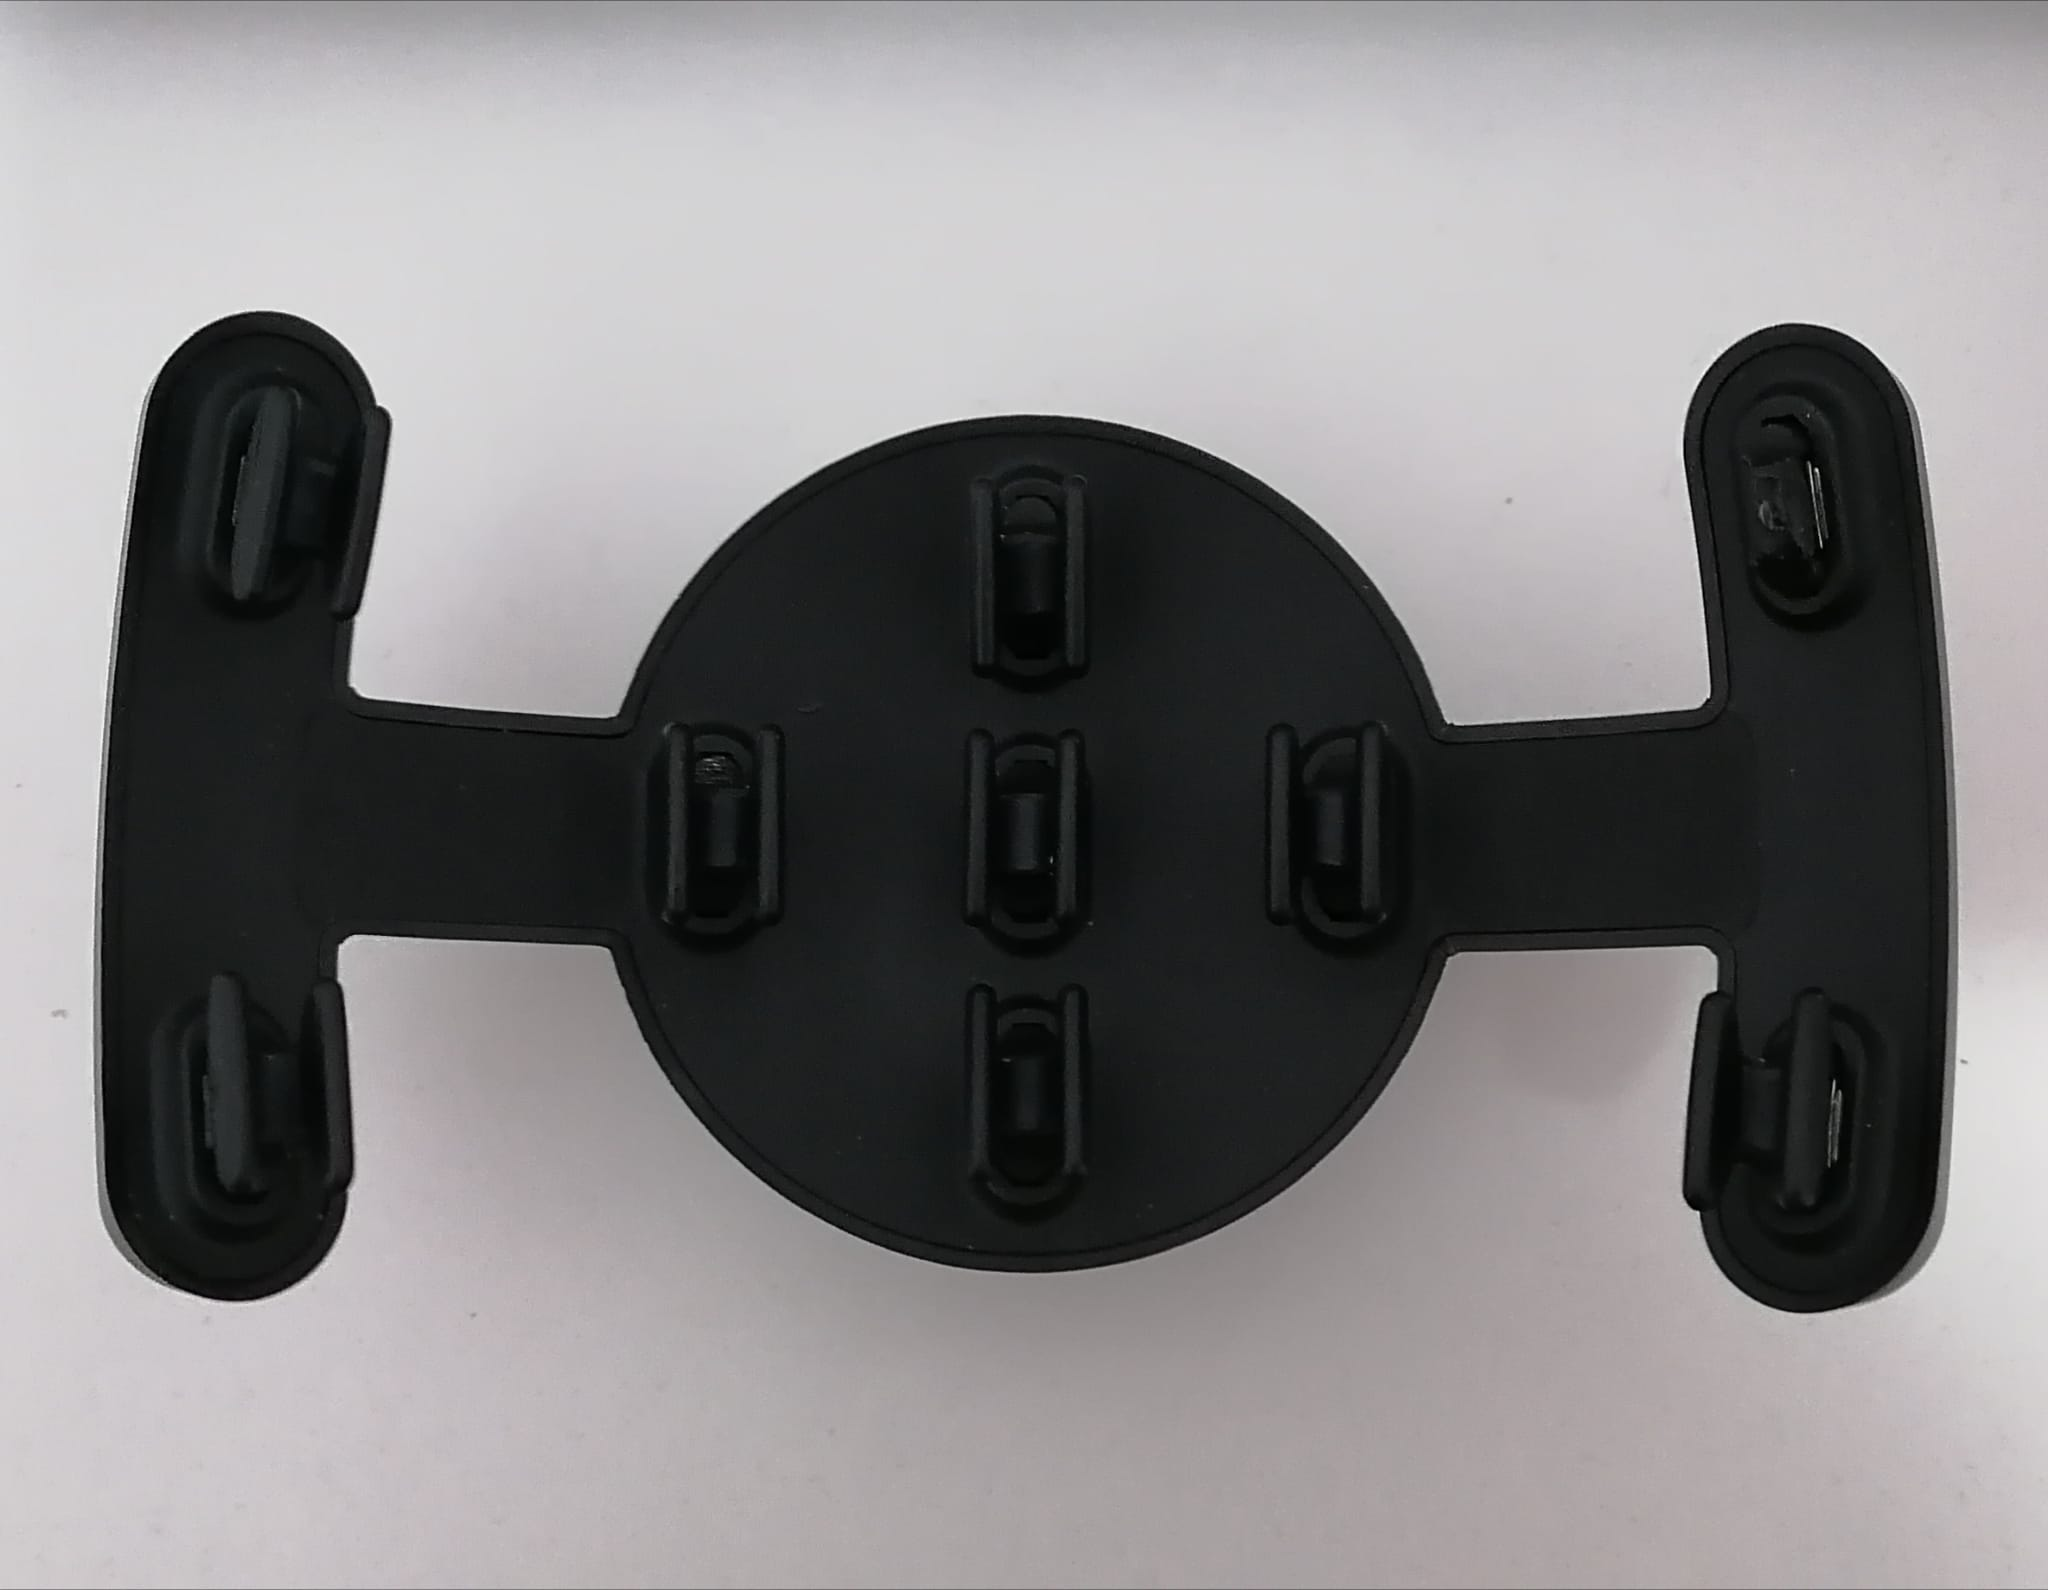
\includegraphics[width=0.5\linewidth]{figures/NextMind electrodes.jpg}
   \caption{Electrodos del casco NextMind}
   \label{figure:nextmind-electrodes}
\end{figure}



Una de las características más relevantes de NextMind es su proceso de encriptación de señales EEG. Al encriptar las señales, NextMind evita que terceros no autorizados puedan interpretar o alterar estas señales. Esta estrategia de encriptación plantea desafíos adicionales en el estudio de de su tecnología, ya que limita la disponibilidad de información detallada sobre su funcionamiento interno.



Estas señales encriptadas son transmitidas vía Bluetooth y sólo pueden ser procesadas a través de la plataforma de desarrollo Unity 3D a través del uso de la SDK proporcionado por el fabricante de NextMind.
